%%
% NCHU Bachelor Proposal Report Template
%
% 南昌航空大学毕业设计开题报告(国内外研究概况和发展趋势)—— 使用 XeLaTeX 编译
%
% Copyright 2023 Arnold Chow
%
% The Current Maintainer of this work is Arnold Chow.
%
% Compile with: xelatex -> biber -> xelatex -> xelatex

\section{国内外研究概况及发展趋势}
国内外关于图像滤波的研究一直是一个发展非常活跃的领域,图像滤波是图像处理中的一项关键操作,
通常在对图像进行处理时都会先对图像进行滤波,已达到消除噪声和其他伪影来提高图像质量的目的。
因此图像滤波的方式非常多,根据不同的
处理要求有相对应的过滤技术。例如常用的高斯滤波器和中值滤波器等,这些滤波器在图像滤波上十
分有效,但因对图像的要求不断提高,这些滤波器已经达不到人们对图像的处理需求,因此各国研究员
根据不同的图像处理需求,开发出了相应的高效滤波器,用来处理各种复杂图像。

在图像过滤中最重要的就是在保留重要的特征的同时降低噪声,这是图像滤波的目的。在很多领域上都
非常热门的神经网络训练在图像滤波上也有发展。PatchShuffle Regularization\cite{kangPatchShuffleRegularization2017}
是一种新的有关卷积神经网络(CNN)的正则化训练,它可以在每个小批量中,随机选择图像或特征图进行转换,
以便对每个局部补丁中的像素进行打乱,可以对噪声的变化更加稳健的过滤,他们在CIFAR-10上实现了5.66\%的
错误率,而不使用PatchShuffle Regularization的错误率为6.33\%。

而在使用深度学习进行图像滤波,Lu\cite{luImageEnhancementUsing2021}等人也提出了一种全新的方法。他们采用了深度学习的全连接神经网络
(FCN)进行图像滤波,其主要工作原理是
在处理噪声像素时会选择前N个邻近的未被破环的像素的候选者来计算灰度等级平均值,用来替换噪声像素,以达到修复的效果。此方法的优势在于
如\ref{07}其他大多数去除噪声的方法在修复噪声像素时仅参考相邻的无噪声像素进行修复,而忽略了噪声图像与无噪声图像的关系,所以导致其重建的质量无法提高。
此方法则可以有效地去除被不同噪声密度损坏的图像中的脉冲噪声。

\begin{figure}[htbp]
	\begin{center}
	    \vspace{10pt} % 调整图片与上文的垂直距离
		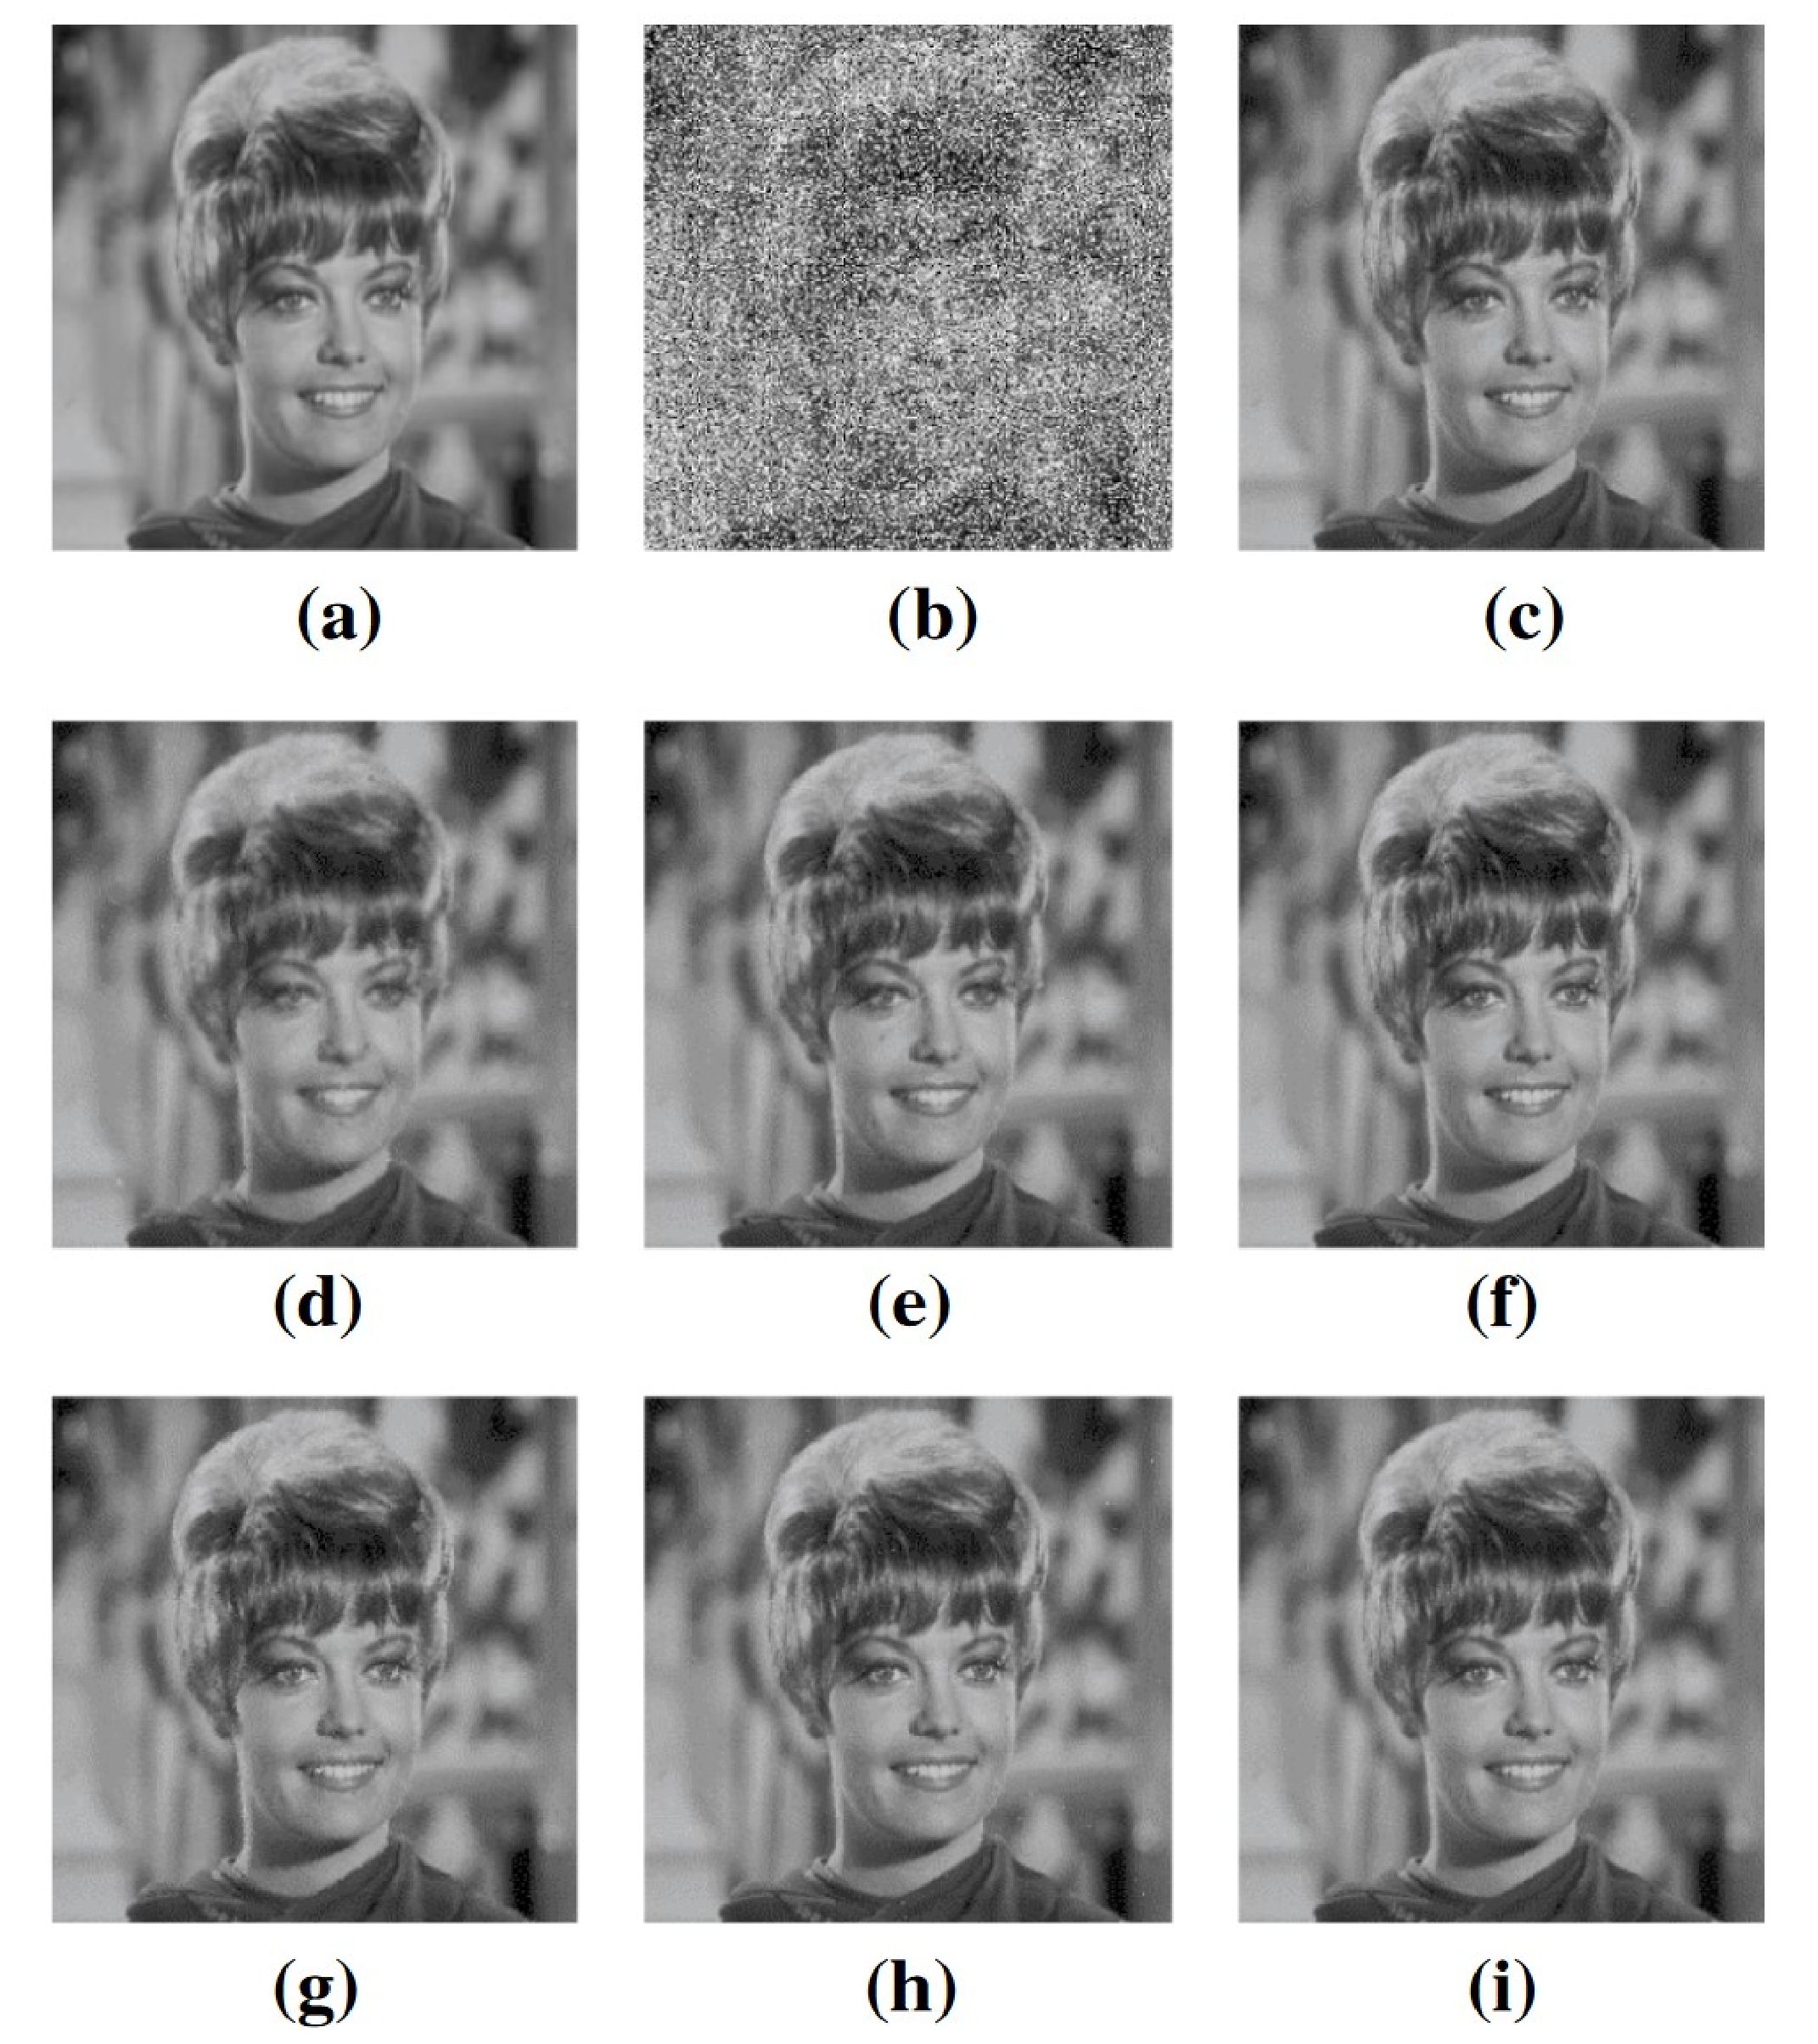
\includegraphics[width = 0.8\textwidth]{images/07.eps}
		\caption{\textbf{a}原始图像;\textbf{b}噪声密度为50\%的噪声图像;通过使用\textbf{c} CNN均值过滤器;\textbf{d} DWM过滤器;
		\textbf{e} MDWM过滤器;\textbf{f} LGII过滤器;\textbf{g} MDW过滤器;\textbf{h} MDBUTM过滤器;\textbf{i}拟议的深度学习FCNN均值过滤器修复的图像。} 
		\label{07} % label 用来在文中索引
	\end{center}
\end{figure}


但是在去除噪声过程不可避免会出现损坏的像素点,所以Satpathy等人\cite{satpathyAdaptiveNonlinearFiltering2022}
提出一种基于决策的非线性算法,它可以同时进行两个操作,即检测损坏的像素和评估新的像素以替换损坏的像素。在不破坏边缘和细节的情况下,实
现了对这些伪像的去除,并在噪声过大时切换到均值滤波,实现了一个算法取代多个算法,提高了效率。

图像过滤中还需要注意不能将对比度损坏,因此Balakrishnan等人\cite{natarajanContrastEnhancementBased2022}提出退化阈值图像检测(DTID)框架,
其使用一个快速双边过滤过程来过滤图像的边缘,以改善边缘过滤图像的对比度。此方法与GUMA、HMRF、
SWT和EHS相比,DTID框架在对比度图像上花费的过滤时间减少了54\%,平均对比度增强质量提高了27\%。与最
先进的方法相比,它提高了28\%平均对比度增强质量、检测准确率26\%并且减少30\%对比度图像的过滤时间。
实际对比见图\ref{03}。

而滤波器中通常为单向滤波器,但是在图像处理中,图像的特征是双向的,所以在降噪过程中就会出现相位失真
而损伤图像特征。因此在图像处理中,双向滤波器是非常重要的,双向滤波器的应用非常广泛,例如图像去噪、
边缘检测和图像分割等。所以Tu等人\cite{tuTwoWayRecursiveFiltering2021}提出了一种双向递归滤波,此方法为了计算一个像素的过滤值,会从相邻的垂直和
水平的像素获得反馈,这样就可以保证图像的特征不会丢失,并减少过滤图像所需迭代次数。其也可以作为在深度神经网络
的一层。如图\ref{01}在实际实验中,该方法在图像去噪和边缘检测上都取得了很好的效果。

\begin{figure}[htbp]
	\begin{center}
	    \vspace{10pt} % 调整图片与上文的垂直距离
		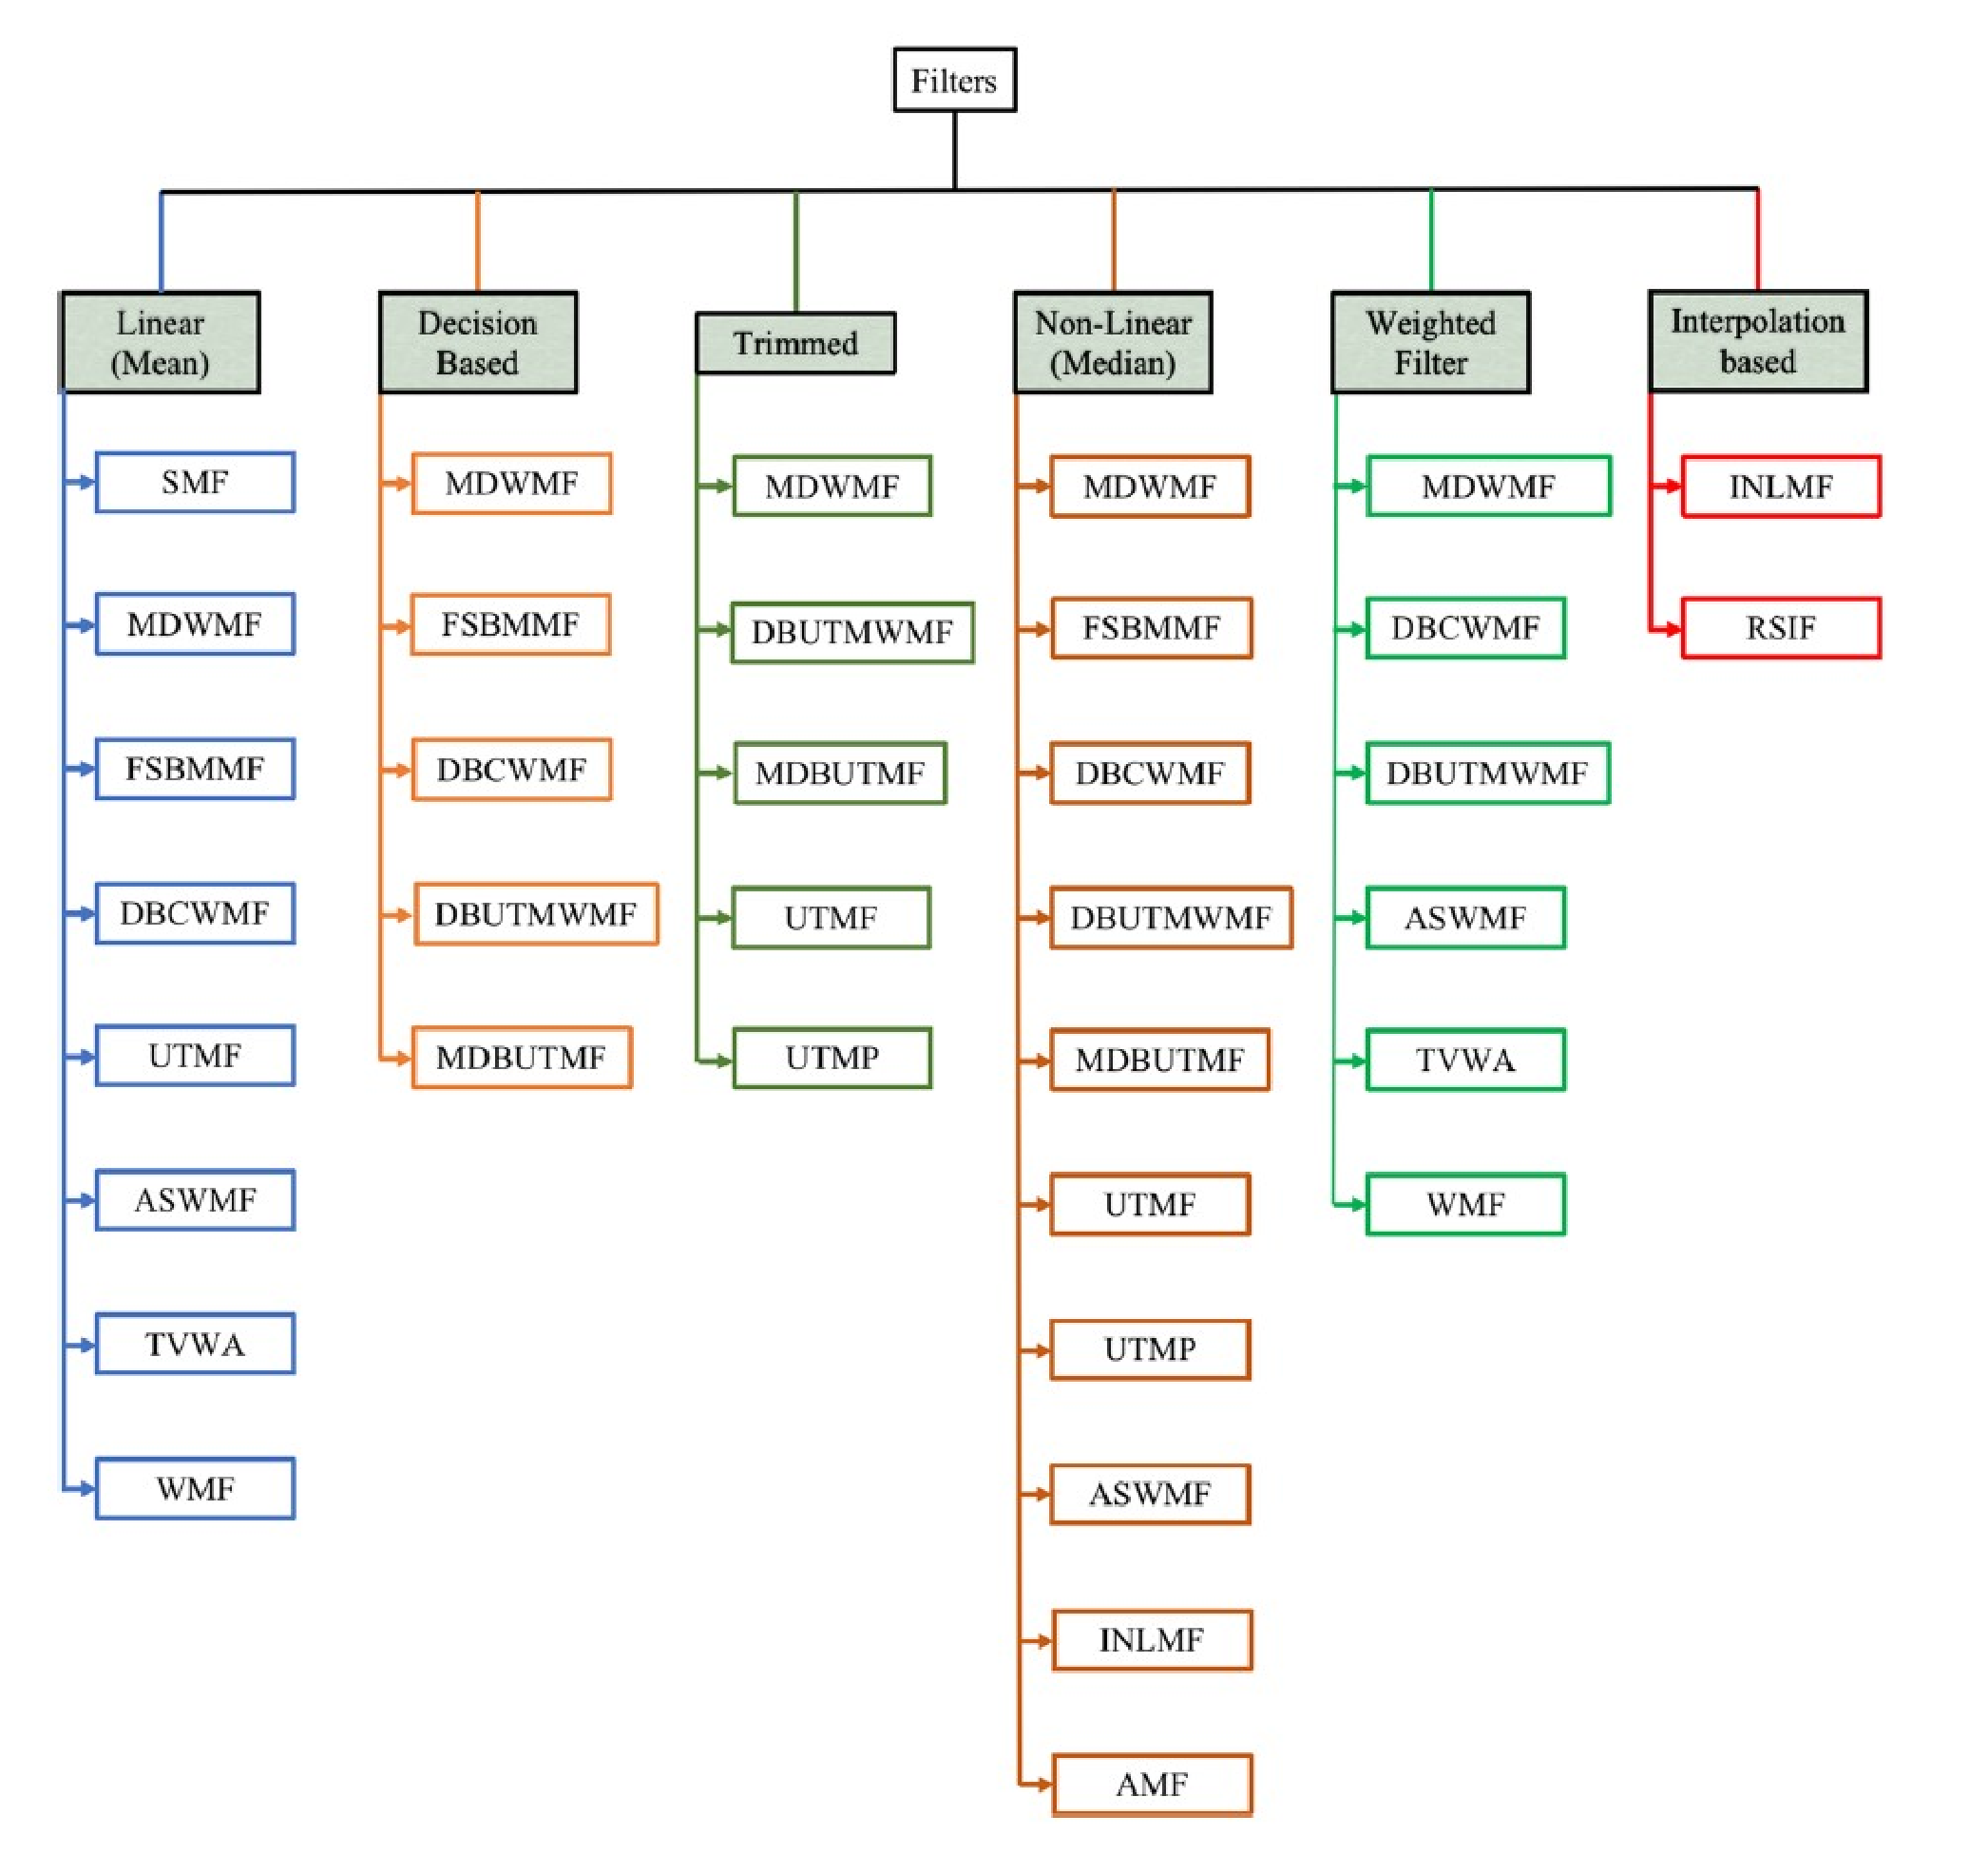
\includegraphics[width = 1\textwidth]{images/01.eps}
		\caption{过滤强度$\sigma$的影响。我们使用不同的过滤强度$\sigma$显示结果。图像平滑度随着$\sigma$的增加而增加,而边缘在滤波后得到很好的保留。} 
		\label{01} % label 用来在文中索引
	\end{center}
\end{figure}

有关贝叶斯方法是一种统计框架其核心是通过新的内容更新先前的内容,其具有连贯性和灵活性,并且在图像处理上也有很好的应用。
所以有很多研究者都在研究如何将其更好的应用在图像去噪上。例如Pablo等人从贝叶斯推理的角度提出了一种新型的非参数降噪技术(FBADA)
\cite{sanchez-alarconFullyAdaptiveBayesian2022},它会自动改善
处理数据的信噪比,并反复评估其平滑版本,通过将信号的期望值计算为整个平滑模型集的加权平均值,就可以做到在无需进行任何参数调整就可以与标准图像
处理算法相媲美,而后者的参数已根据要恢复的真实信号进行了优化,这在实际应用中是不可能的。其对极度嘈杂(高于 20-40\%的相对误差)的信号重建得到
的残差的标准偏差可能会比原始测量的标准偏差低一个数量级以上。图\ref{02}为其处理不同噪声的效果图。

\begin{figure}[htbp]
	\begin{center}
		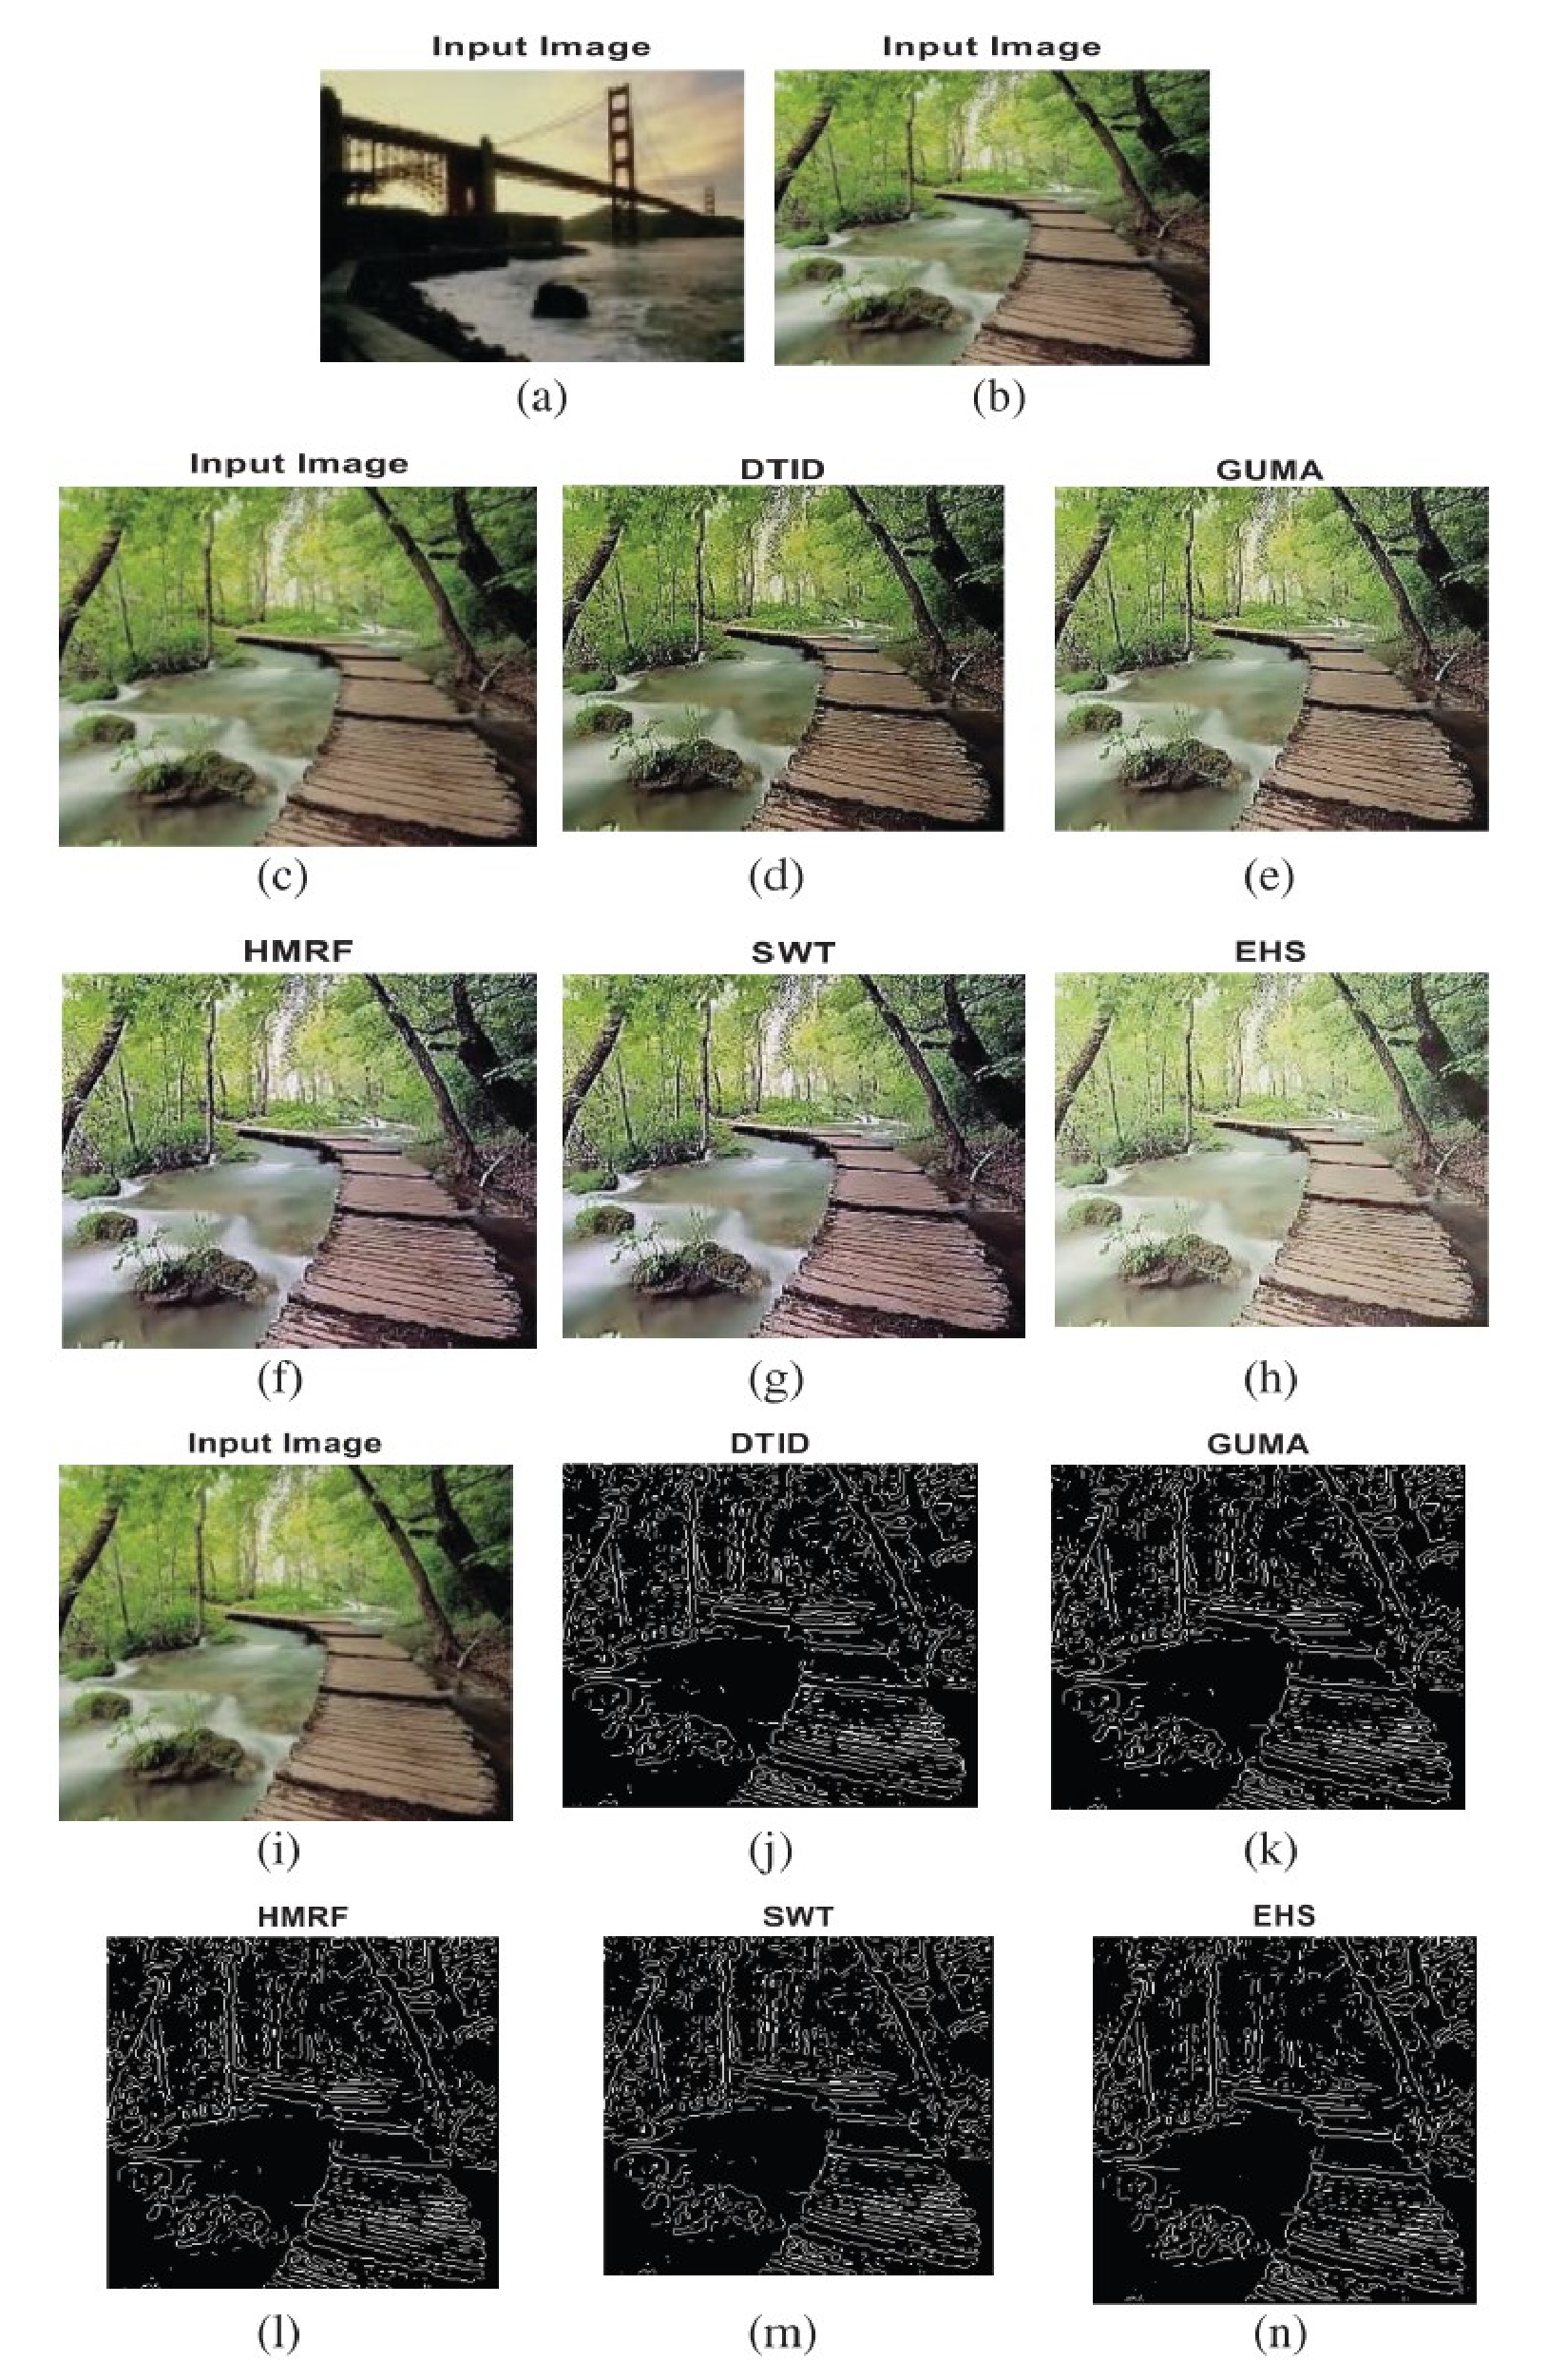
\includegraphics[width = 0.8\textwidth]{images/03.eps}
		\caption{使用DTID、现有的GUMA、HMRF、SWT和EHS对平均对比度增强质量和检测准确率的定性分析。
        (a) 输入图像1 (b) 输入图像2 (c) 输入图像 (d) 使用DTID的对比度增强质量 (e) 使用GUMA的对比度增强质量 
        (f) 使用HMRF的对比度增强质量 (g) 使用SWT的对比度增强质量 (h) 使用EHS的对比度增强质量 
        (i) 输入图像 (j) 使用DTID的检测准确率 (k) 使用GUMA的检测准确率 (l) 使用HMRF的检测准确率 
        (m) 使用SWT的检测准确率 (n) 使用EHS的检测准确率} 
		\label{03} % label 用来在文中索引
	\end{center}
\end{figure}

在图像滤波的领域上存在复合型滤波器,他通常会结合多个滤波器的特点,例如在图像去噪中,可以结合高斯滤波器和中值滤波器,
这样就可以保证图像的平滑性和边缘的保留。所以复合型滤波器也是图像滤波的研究热点之一。而其中增强型滤波器就结合了维纳滤波器和
频谱减法技术以提高降噪和信号增强性能。首先,应用维纳滤波器估计输入信号的功率谱密度和噪声。然后,利用频谱减法技术估计噪声的功率谱密度,
从输入信号的估计功率谱密度中减去该功率谱密度。最后,再次将维纳滤波器应用于修改后

\begin{figure}[htbp]
	\begin{center}
		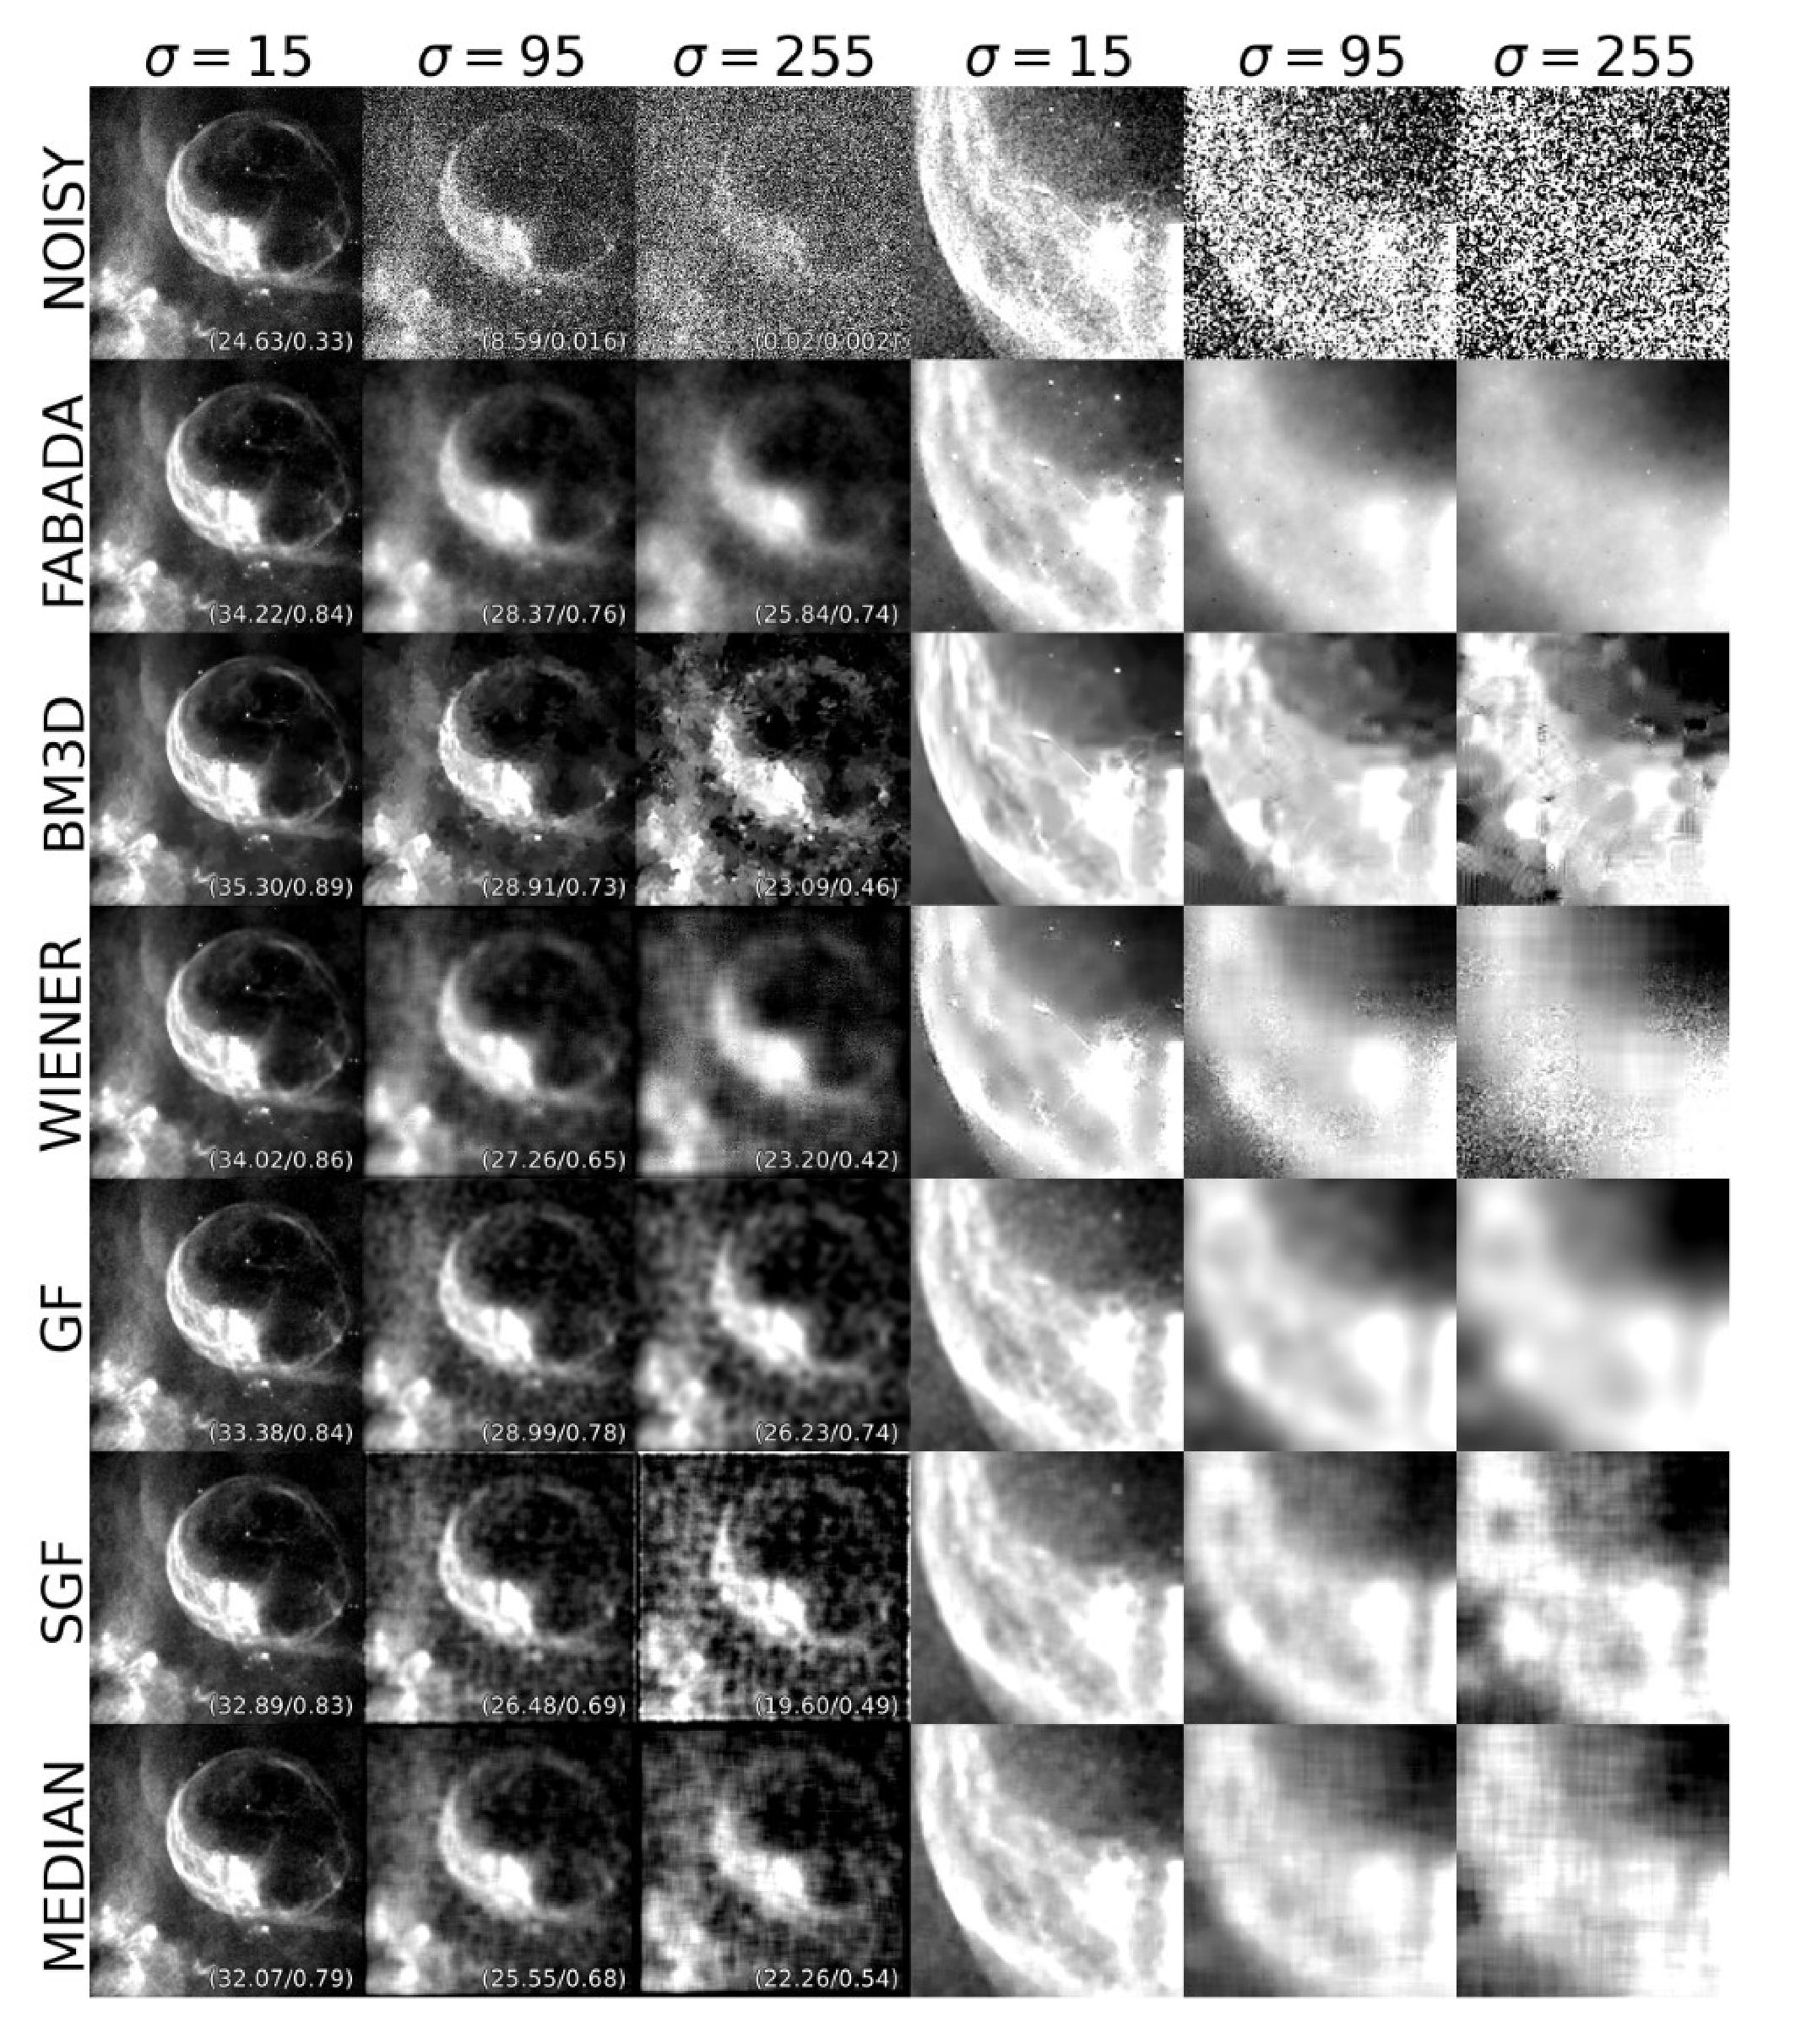
\includegraphics[width = 0.85\textwidth]{images/02.eps}
		\caption{气泡图像的估计结果示例,显示三个不同噪声值($\sigma$ = 15、95、255)的恢复,即 PSNR 值
        (24.63、8.59、0.02)dB 和 SSIM(0.33 , 0.16, 0.002).行和列分别代表不同的算法和噪声级别,如标签所示。最后三列显示了气泡结构的特写,以更好地衡量精细细节的恢复情况。} 
		\label{02} % label 用来在文中索引
	\end{center}
\end{figure}

\noindent 的功率谱密度以产生增强信号。其高降噪性能和计算复杂度低等优点
使其应用非常广泛。所以Pranay在2019年提出了一种新的增强型滤波器\cite{kumarImageDeNoisingSalt2019}。其相对于其他滤波器对低、中密度的固定值
脉冲噪声有更好输出,该方法的主要使用修剪后的平均值取代噪声像素,以达到提高峰值信噪比(PSNR)和减少图像模糊的目的。其在实际实验中,能让视觉感更好。

自适应滤波在图像处理上是一个非常重要的研究方向,它可以根据图像的特征自动调整滤波器的参数,从而达到更好的滤波效果。
用来处理各种复杂图片,在实际应用中也是非常有用的。所以各国研究员一直在对如何改进自适应滤波器进行研究。例如Soheila等人提出将非参数知识结合到最小
均方自适应滤波器中(NPLMS)\cite{ashkezari-toussiIncorporatingNonparametricKnowledge2019},此方法在最大后验估计的框架下用于估计来自噪声
数据的未知参数向量,并且使用核密度估计来估计先验分布,但为了对高斯和
非高斯噪声具有鲁棒性,一些中间估计被缓冲,然后用于估计先验分布,在有偏置补偿算法也不需要估计输入噪声方差,以此得出了NPLMS。此外,还提供了 NPLMS 的可变步长
版本以减少稳态误差。

在图像过滤领域中,最重要的是制定有效的过滤规则,其为过滤性能的关键所在。目前设计的内核平移不变的过滤器已被广泛使用,但是它们的性能容易被内容盲区
影响,进而影响过滤性能。所以一个被称为联合/引导过滤器的过滤器系列引起了广泛关注,在同一场景的多个图像中包含可用于减少噪点和增强细节的互补信息。
这在单个图像有噪点或对比度低的情况下特别有用。

\begin{figure}[htbp]
	\begin{center}
	    \vspace{10pt} % 调整图片与上文的垂直距离
		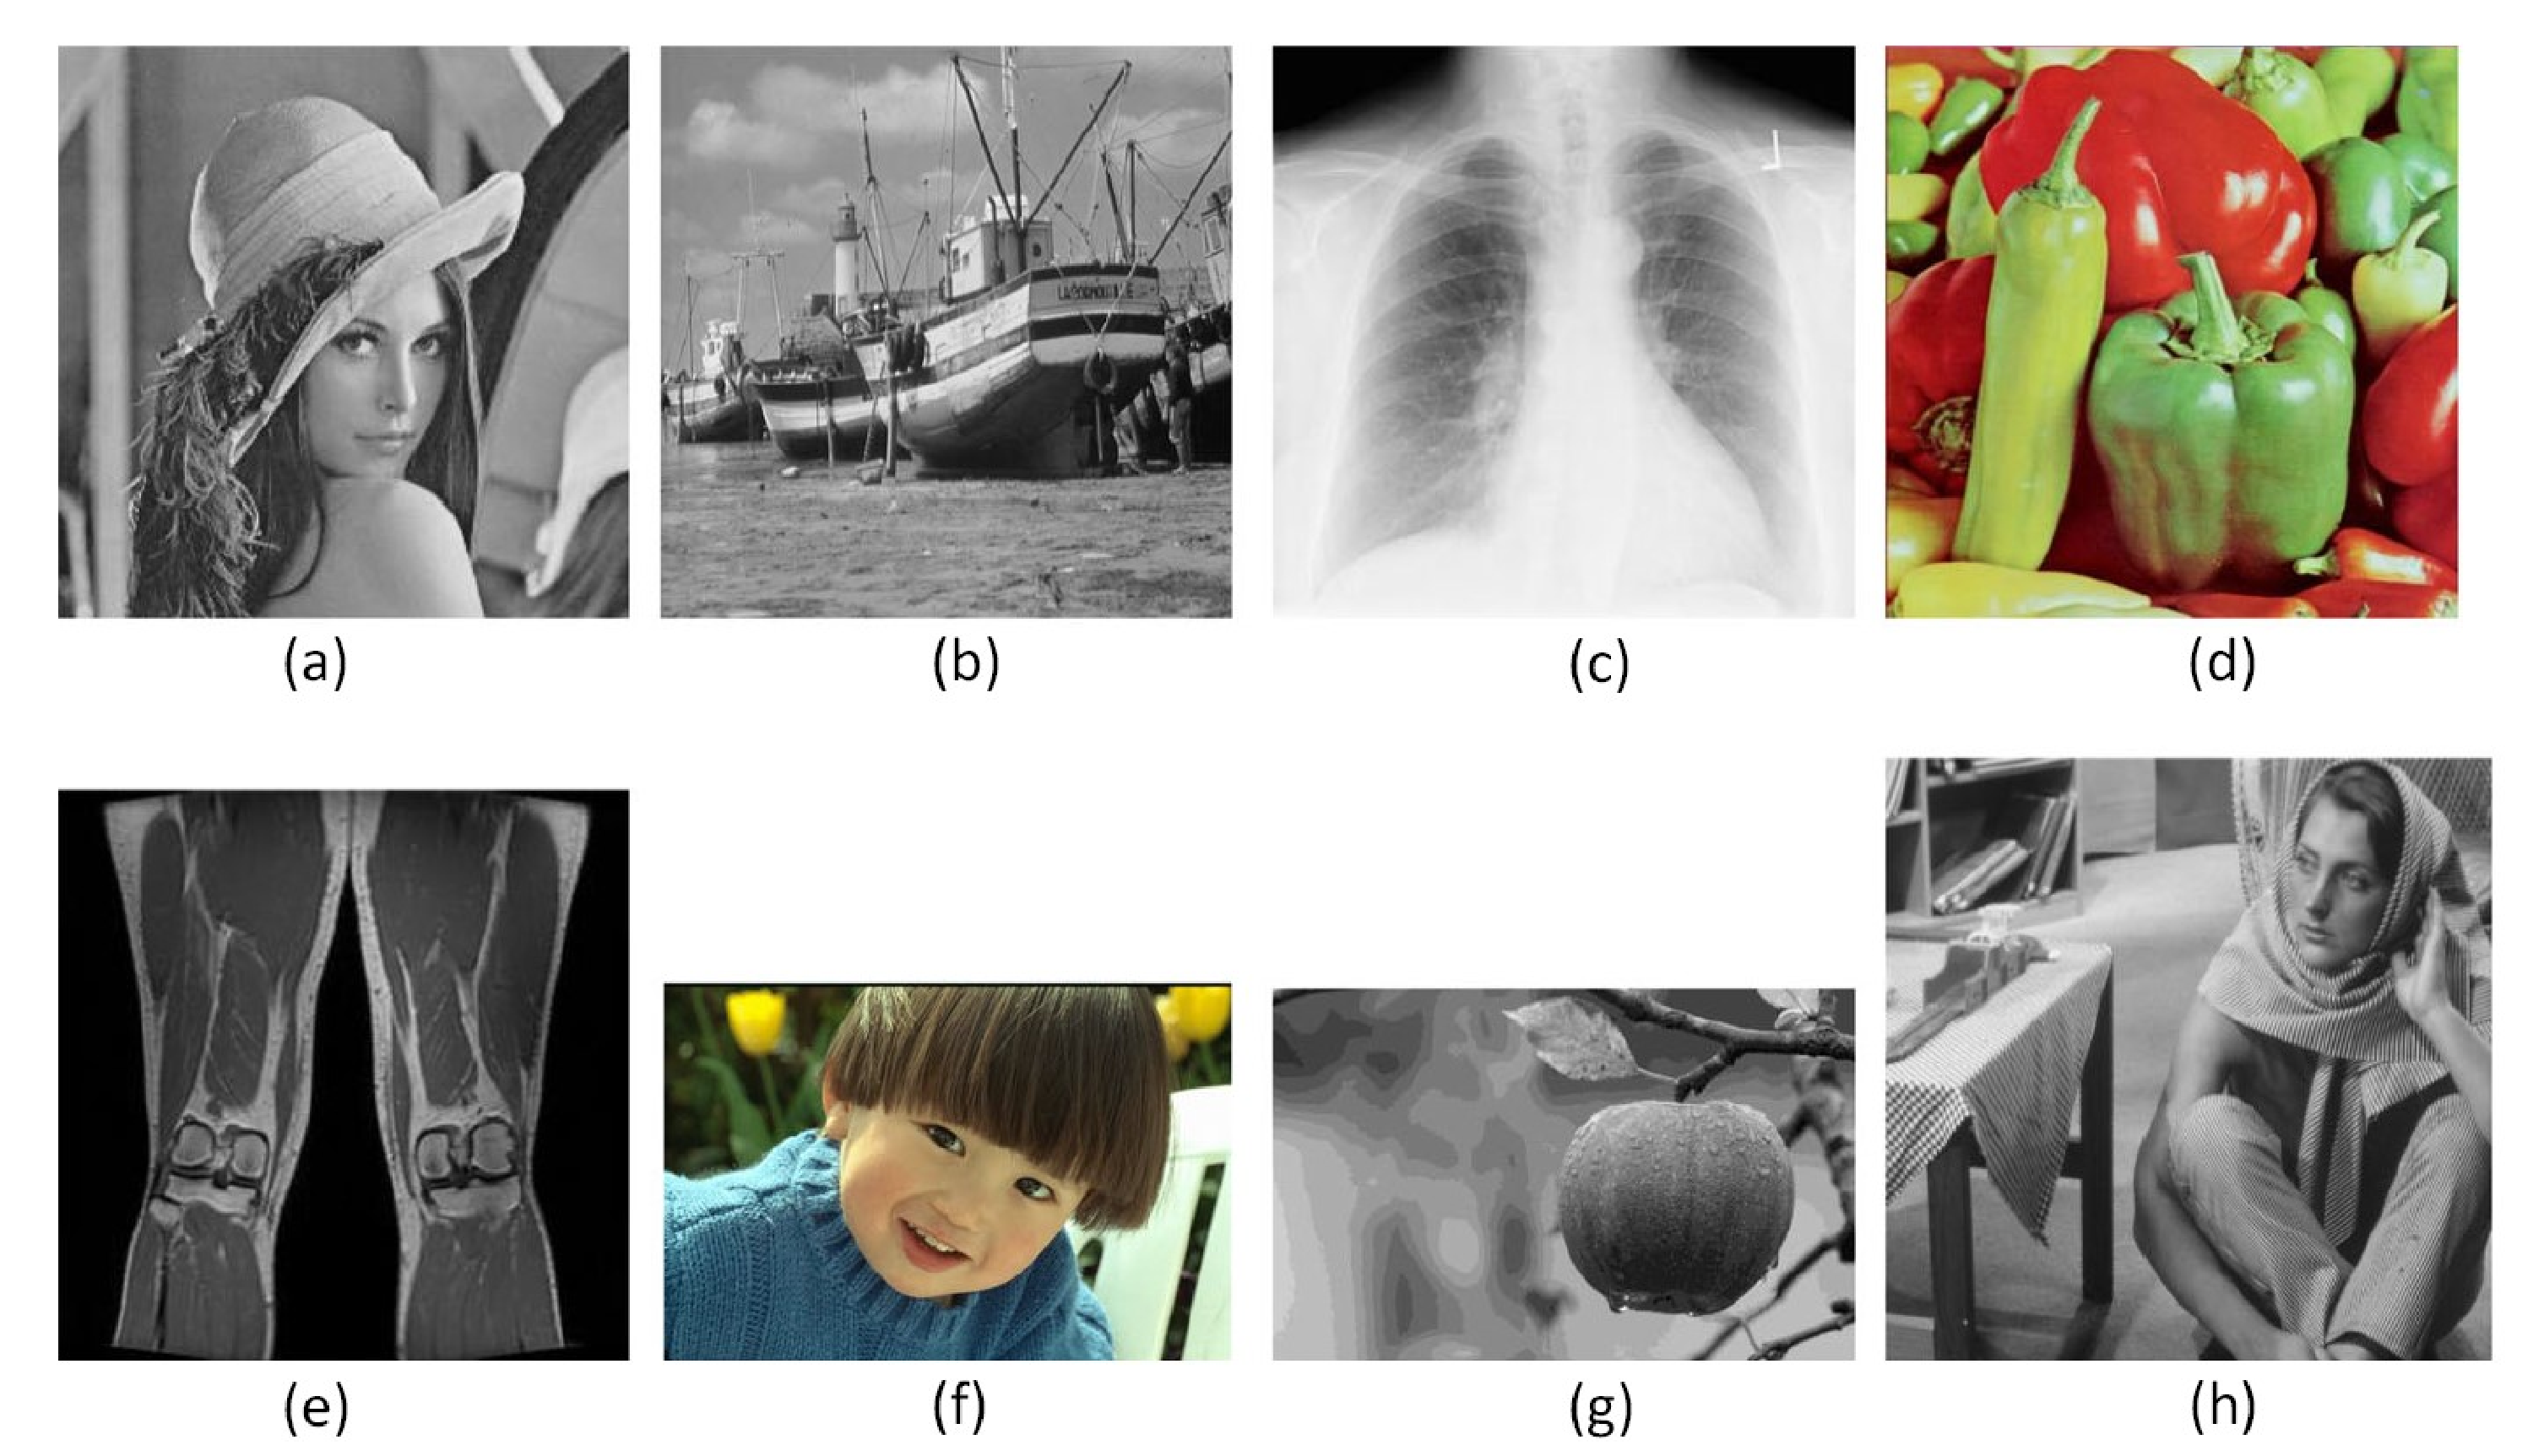
\includegraphics[width = 1\textwidth]{images/04.eps}
		\caption{关于相互结构提取的视觉比较。(a)和(b)分别是白天和晚上的图像。(c)和(d)是JFMS的结果
        ($\epsilon_{I}=\epsilon_{G}=2e-4$和$\lambda_{I}=\lambda_{G}=1$)。(e)和(f)是muGIF的结果(在$\alpha_{t}=\alpha_{r}=0.03$)。
        (g)和(h)是muGIF的结果(在$\alpha_{t}=\alpha_{r}=0.06$时)。} 
		\label{04} % label 用来在文中索引
	\end{center}
\end{figure}

但其主要缺点来自于对参考信号和目标信号之间结构不一致的忽视,如在不同条件下拍摄的彩色、红外和深度图像。简单地
采用这种准则很可能导致不满意的结果。为了解决上述问题,Guo等人提出了相互引导图像滤波器(muGIF)\cite{MutuallyGuided2020},如图\ref{04}它能保留共同的相互结构,
避免不一致结构的误导,并使平坦区域变得平滑。其方法非常灵活,可以在自我引导,参考引导,和相互引导之间切换,其有效性和灵活性都得到了验证。
但是在某些方面也存在局限性当RGB图像被破坏时,特别是在微小的结构上,即使有另一种辅助手段(如近红外),修复后的结果也不能满足。并且类似半色调
的情况精确定位边缘的优势反而成为劣势。

而有关联合/引导过滤器的过滤器系列可以对输入图像执行边缘保留平滑,如导引图像滤波(GIF)和加权导引图像滤波(WGIF)其可以保留图像的细节和边缘,
同时去除噪声,而且不会产生锯齿状边缘。这使得它们在保留图像的结构和细节特别有用。但是其仍有主要缺点是不能保留精细结构,为了解决以上问题,
Li等人提出了一种新的全局引导图像滤波(G-GIF)\cite{SingleImageDeHazingUsingGloballyGuidedImageFiltering2018},由一个全局结构转移滤波器和
一个全局边缘保留平滑滤波器组成。用于对图像进行雾霾去除处理,如图\ref{05}结果表明所提出的除霾算法确实提高了除霾图像的视觉质量,产生更清晰的图像,并能明
显更好地保留精细结构区域的细节。

\begin{figure}[htbp]
	\begin{center}
	    \vspace{10pt} % 调整图片与上文的垂直距离
		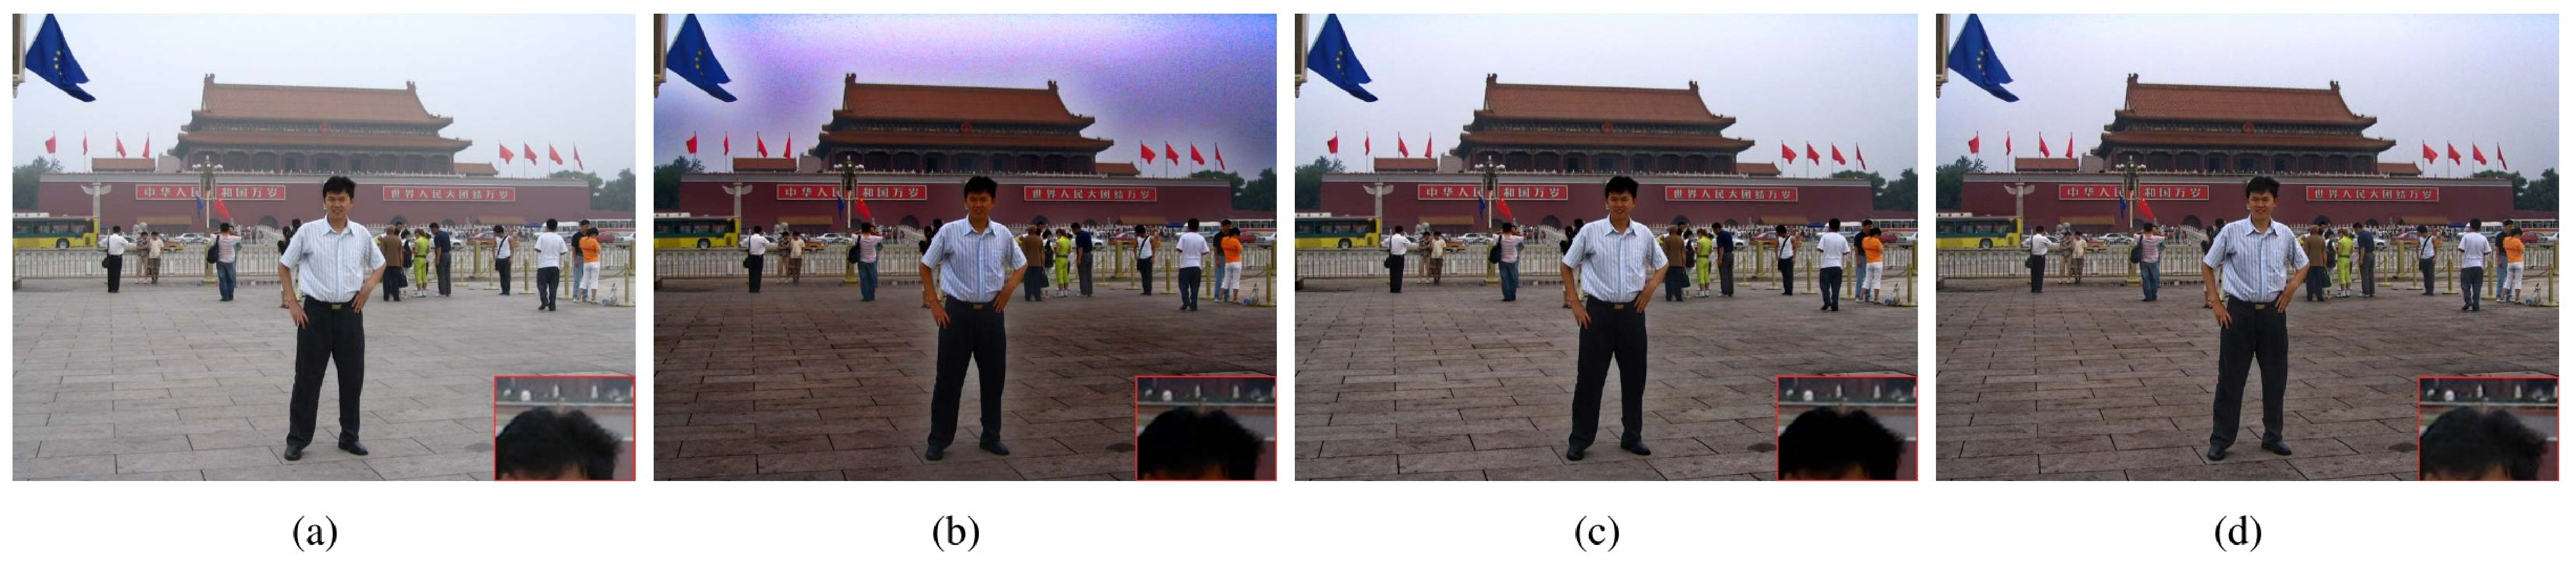
\includegraphics[width = 1\textwidth]{images/05.eps}
		\caption{GIF、WGIF和G-GIF的比较。(a) 雾霾图像;(b) GIF的除霾图像;(c) WGIF的除霾图像;(d) G-GIF的除霾图像。GIF和WGIF都对人类主体
        的头发进行了过度平滑处理,如放大区域所示,而所提出的G-GIF则克服了这个问题。} 
		\label{05} % label 用来在文中索引
	\end{center}
\end{figure}

均值滤波也是常用的图像滤波的方法,针对不同的场景分为很多类别,其中非局部均值滤波(NLM)算法是其中一种,它可以在保留图像细节的同时去除噪声。
但是NLM算法的计算量较大,而且方形搜索窗口会将大量低相似度的图像块引入去噪图像的加权平均计算过程中, 导致去噪图像的细节轮廓变得模糊.因此在
萧澍等人\cite{xiaoTuoyuanchuangkouhecanshuzishiyingdefeijubujunzhisuanfa2020}
提出了可以利用控制核函数来获取椭圆窗口和图像块参数的自适应 NLM 算法。通过相关信息获得描述图像局部边缘结构的椭圆方程以此确定窗口形状,然后搜索
椭圆形图像块,并用自适应平滑参数来增强算法效果。实验表明在其PSNR和SSIM值相比于传统的NLM相关算法更高,并且随着噪声等级提升其可以在抑制噪声的同时
能更好的保留高频纹理信息。图\ref{06}为四种方法对四种方法去噪效果对比图。

\begin{figure}[htbp]
	\begin{center}
		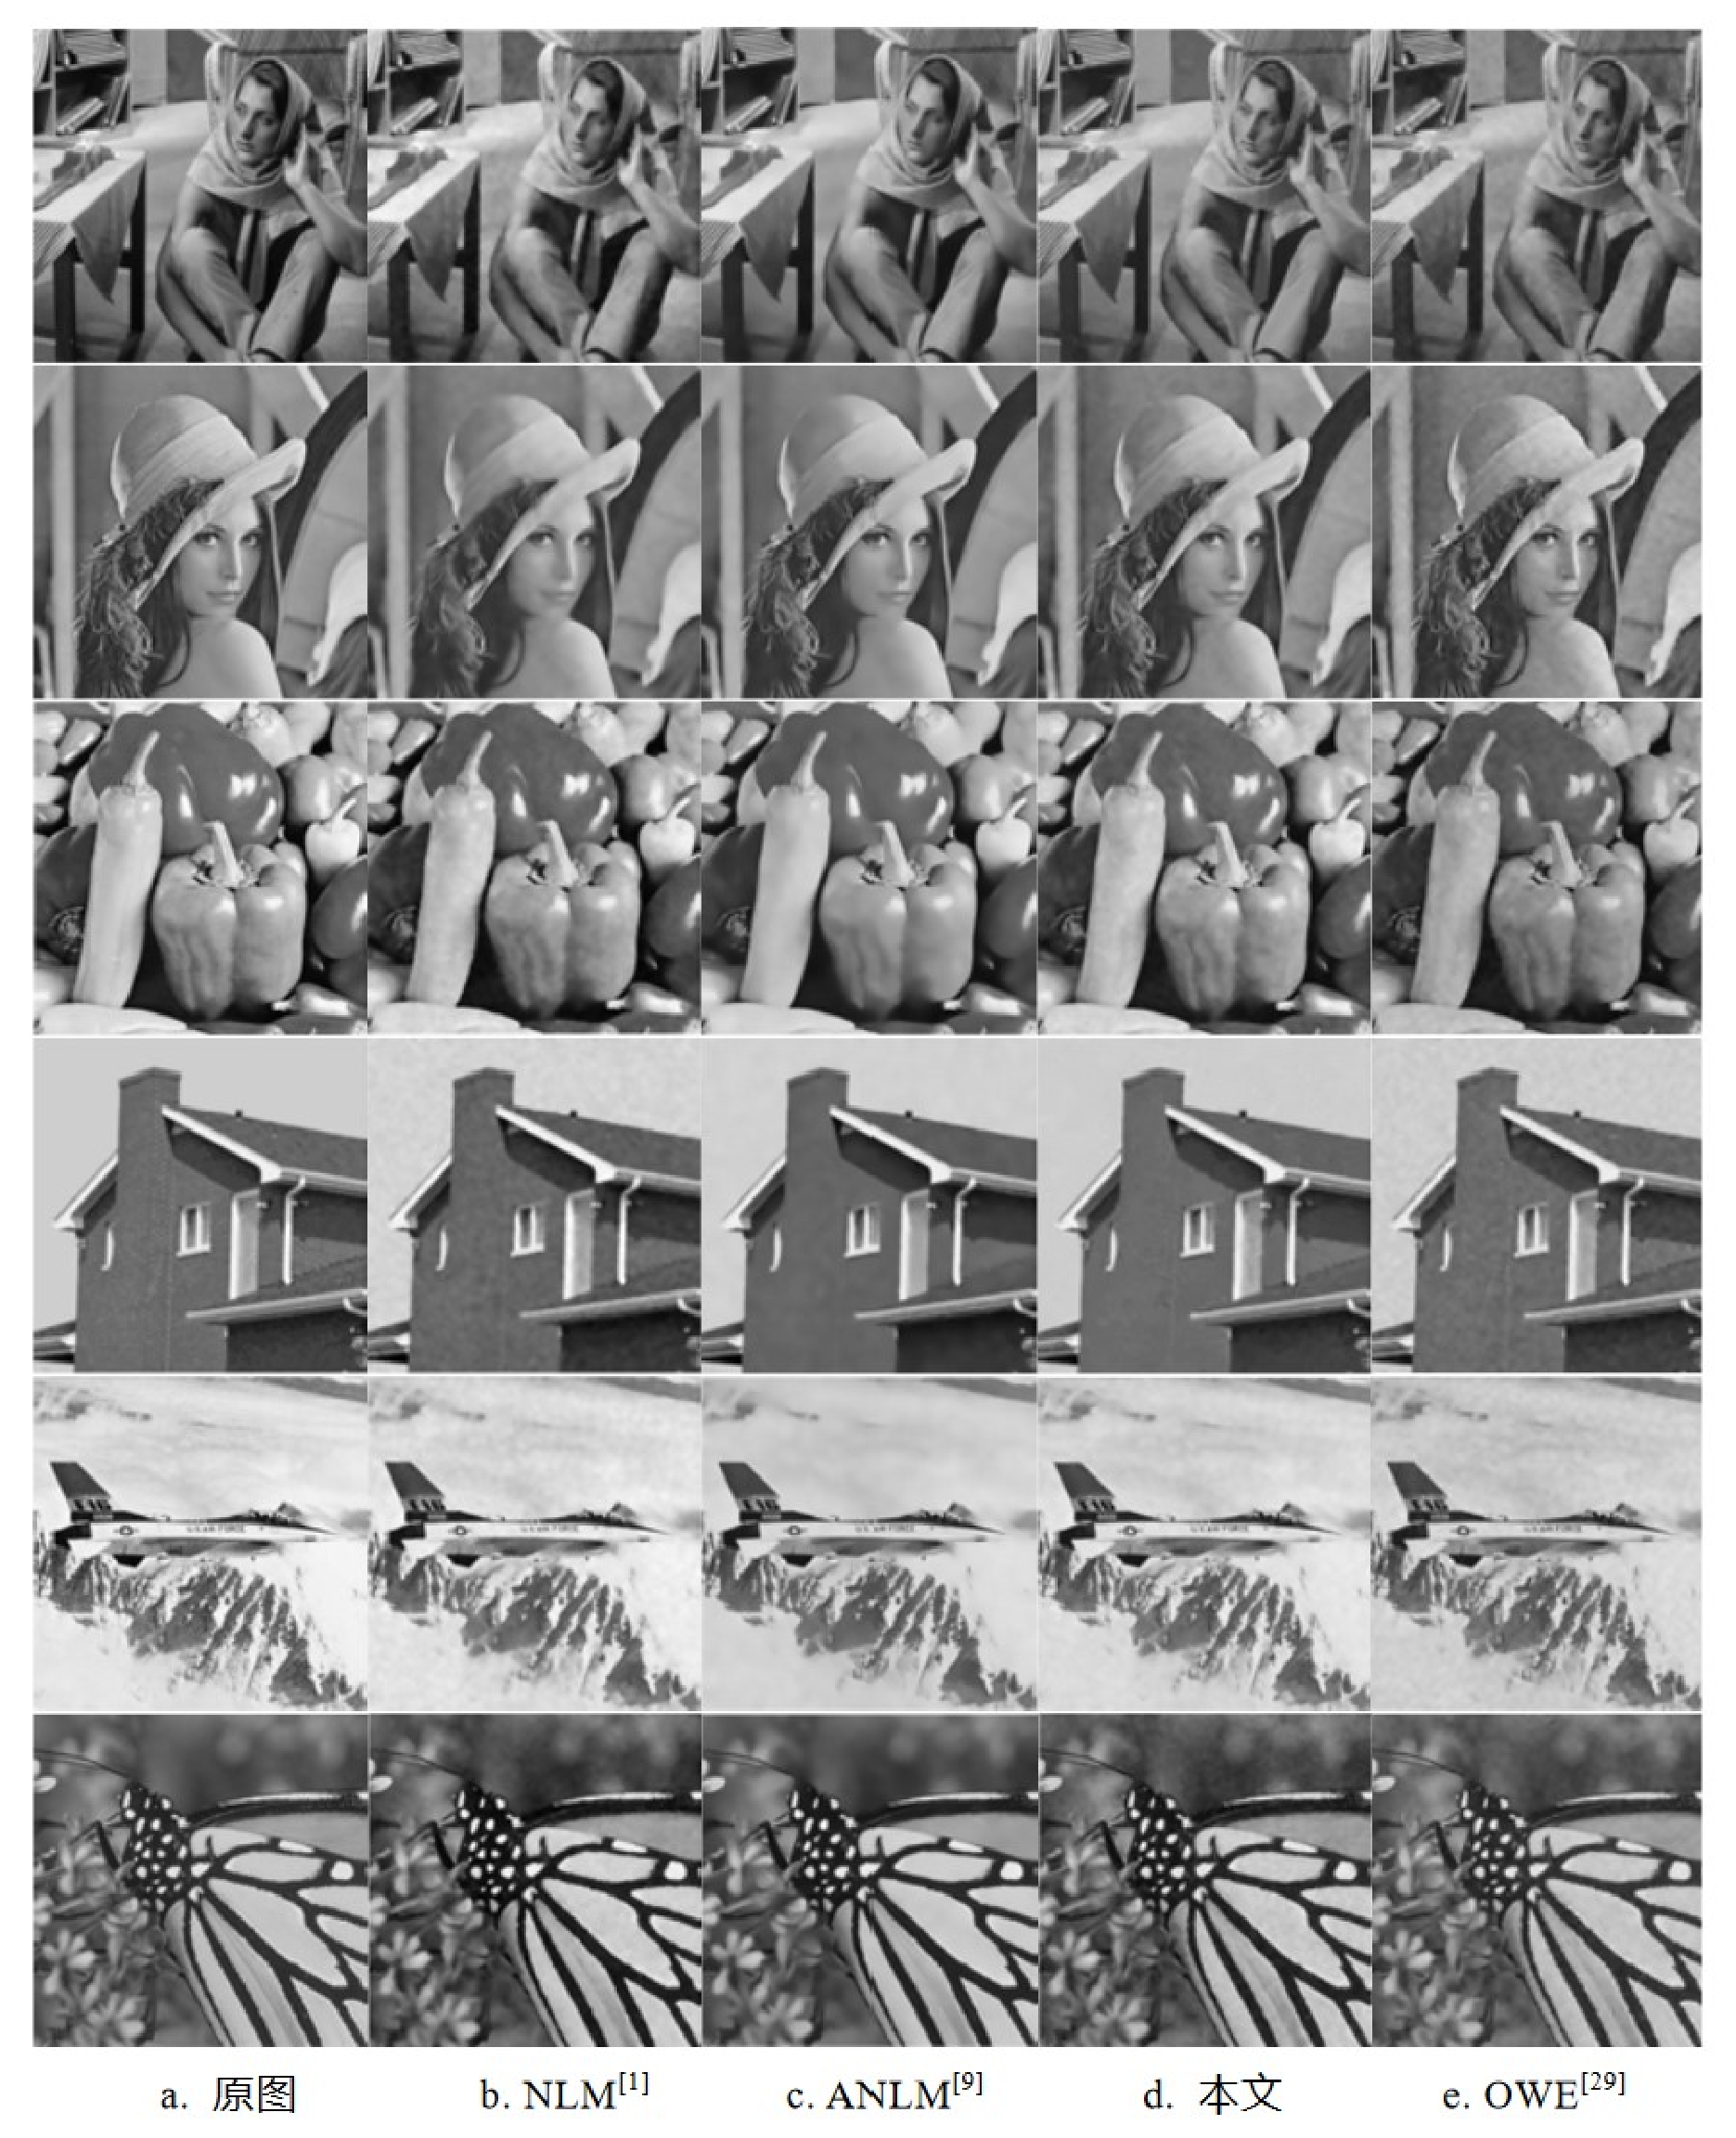
\includegraphics[width = 1\textwidth]{images/06.eps}
		\caption{4种算法对 $\sigma=30$ 的噪声图像处理后的去噪效果图} 
		\label{06} % label 用来在文中索引
	\end{center}
\end{figure}

双边滤波可以识别显著的边缘细节,并且保留几何信息,同时还具有容易实现等优点,但随着噪声变大,其抑制噪声的能力就会变差,而加权双边滤波则因采取了
均值滤波而导致会丢失一部分纹理,所以秦毅等人\cite{qinJieheCurveletbianhuanyujiaquanshuangbianlubodetuxiangquzaofangfa2021}提出了
结合Curvelet变换与加权双边滤波的混合域图像去噪方法,其通过将加权双边滤波器将噪声图像分解为低频部分和高频部分并对高频部分使用Curvelet变换的折衷阈值
进行处理以保留细节,最后再将两者重构。该方法使得对于峰值信噪比(PSNR)等相关指数有实质性的提高。

% (含文献综述)
% 该部分主要需要写:
% \begin{enumerate}[label=\arabic*)]
%     \item 要实现研究目标,要使用哪些方法、系统、工具和技术?国内外研究现状、发展动态如何?
%     \item 是否还有其它方法、系统、工具和技术?分析、比较它们各自有哪些优缺点?
% \end{enumerate}
% 这就需要大家多阅读文献。关于文献还需要注意:
% \begin{enumerate}[label=\arabic*)]
%     \item 是否多为近3-5年的参考文献,且来自本领域的主流期刊?
%     \item 参考文献的引用格式是否规范?(\sout{都使用这套模板了,那肯定没问题的啦})
% \end{enumerate}
